Encuentra el valor de la incógnita en el triángulo de la figura \ref{fig:angle_triangle_34}.

\begin{minipage}[t][][t]{0.35\textwidth}
    \begin{figure}[H]
        \centering
        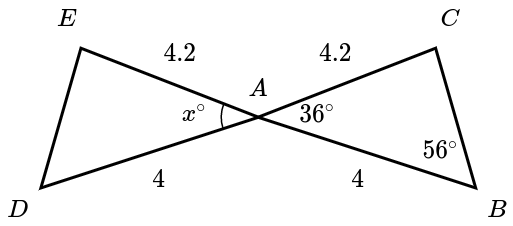
\includegraphics[width=0.9\linewidth]{../images/angle_triangle_34.png}

        \caption{}
        \label{fig:angle_triangle_34}
    \end{figure}
\end{minipage}\hfill
\begin{minipage}[t][][t]{0.6\textwidth}
    \begin{solutionbox}{3cm}
        $\angle DAE$ forma un ángulo opuesto por el vértice con $\angle BAC$, por lo tanto la medida de
        $\triangle DAE$ es igual a la medida de $\triangle BAC$.
        $\triangle ABC$ y $\triangle ADE$ también tienen dos lados iguales. Por lo tanto,
        $\triangle ABC$ y $\triangle ADE$ son congruentes.
    \end{solutionbox}
\end{minipage}
